\chapter{Mathematical Model}

\bigskip
\noindent A.G Streng and A.V. Grosse \cite{Streng}  studied the ozone oxygen flame experimentally. The stability of ozone and the rates of decomposition or explosion were investigated by Armour research foundation. Ozone was burned to oxygen from a simple burner tip in the range from 17 percent to 100 percent initial concentration of ozone in the mixture. The flame temperatures were calculated from enthalpy data and dissociation constants of oxygen using kelley's tables. The concentration of ozone was kept constant with error of   0.2 percent. Two methods were used to determine burning velocity i.e open tube method and the burning tip method. We will be using experimental burning velocity of the burning tip method. The burner tip experiments were carried out in standard apparatus, using pyrex glass aluminium tips with an inner diameter of 3 to 0.65mm. The flames were readily observed by the standard schlieren method at all concentrations above 30 mole percent. The measurements were all carried out in the laminar flow region and the reynolds number of the flow was below 2000. The initial conditions are 300K temperature and 1.0 atmosphere pressure. The results of burning velocities of ozone flames were compared with theoretical burning velocities of Dr. Von Karman and his associates. They were found to be in close agreements. 

\section{Governing Equations}


The final equation obtained by from asymptotic analysis is given below. These quantities are non dimensionalised. 
\begin{eqnarray}
-\nabla \cdot u &=& \frac{1}{p^0} \frac{d p^0}{d t} - \frac{1}{T}\frac{D T}{D t} \hspace{1mm}\\
\rho \frac{D u}{D t} \hspace{1mm} &=& -\frac{1}{M^2}\hspace{1mm}\nabla p\hspace{1mm}+\hspace{1mm}\frac{1}{Re}\nabla \cdot \tau + \frac{1}{Fr^2}\rho g \\
\rho C_p \frac{D T}{D t} \hspace{1mm}&=&\hspace{1mm} -  \frac{1}{Re Pr}\nabla\cdot (k \nabla T) + \hspace{1mm} \frac{1}{\gamma -1} \frac{d p^0}{d t}\hspace{1mm}\\
\end{eqnarray}



\noindent The species conservation equation is given as 
\begin{eqnarray}
	\frac{\partial \rho_i}{\partial t} + \nabla . (\rho_i v) &= \nabla . (\rho D_{ij} \nabla Y_i) + w_i
\end{eqnarray}
\noindent Where, the rate of production for species $i$ is given by the following 
	
Where $$w_i = Mw_i \sum_{k=1}^{6}(v_{k,i}^{''} - v_{k,i}^{'}) B_k T^{\alpha_k} e^{\frac{-E_a}{R_u T}} \prod_{j=1}^3 \left(\frac{X_j p}{R T} \right)^{v'_{j,k}}$$

\noindent The above equation considers all reactions for all the species. 

\noindent From atomic species conservation 
	$$\sum_{i=1}^{N} v_i{'}M_i \rightleftharpoons \sum_{i=1}^{N} v_i{''}M_i $$
\noindent Where $E_a$ is the activation energy, $R_u$ is the universal gas constant, $X_j$ is the molar concentration of the reactant j, $Mw_i$ is the molecular weight of the reactant. $v'_{j,k}$ is the moles of reactant j in the reaction k. $v''_{j,k}$ is the number of moles of product. 

\bigskip

\noindent The overall continuity equation, species conservation equation and energy conservation equation are solved to calculate the flame parameters. The energy equation considers that the pressure is constant throughout the reaction zone. The viscous dissipation is negligible and there is no body force work. 

\noindent The Diffusion equation is given 
\begin{eqnarray}
\frac{\partial X_k}{\partial x} &= \sum_{j=1}^{3} \frac{X_k X_j}{D_{jk}} (V_j - V_k)
\end{eqnarray}

\noindent Where $D_{jk}$ is the fick's diffusion coefficient. $V$ is the diffusion velocities. 

\noindent The boundaries are defined by specifying the concentration of $O_3$, $O_2$ at the inlet. 

\section{Premixed ozone oxygen laminar flame model}
We shall use Heimerl and coffee's contemporary method for modelling combustion flame problem. A one dimensional, premixed, laminar, steady state ozone oxygen flame was considered in their theortical model. The reason for choosing this model was due to its simplicity. The chemical reactions involved only three species 


			$$O_3 + M \rightleftharpoons O + O_2 + M $$
			$$ O + O_3 \rightleftharpoons A_2  2O_2$$ 
			$$A + AB \rightleftharpoons A_2 + B$$
\noindent Where M represents the third body which could be either $O$, $O_2$ or $O_3$. 


\section{The experimental data on laminar flame speed}

To compare our results we have used the experimental data given by the A.G.  streng and A.V. Grosse, They have done experiments with ozone flame in tube and ozone flame on the tip of the burner. We will be using the results of the later. They have shown that laminar flame speed or burning velocity varies with the initial concentration of the ozone. The table given below shows the burning velocity with respect to initial concentration of the ozone. We concentrate on two speciifc cases where initial concentration of ozone is 53 percent and 100 percent. The laminar flame speed for 53 percent is measured in the burner with inner diameter 1.3mm  and rate of 7.7 cc/sec. The laminar flame speed for 100 percent ozone is taken on .66 inner diameter tip 0.66 mm and the flow rate of 8.23 cc/sec. 
The measured laminar flame speed is given below. Laminar flame measurements are carried out at 300K and 1 atmosphere pressure. 

\begin{table}[h]
\caption {Experimental laminar flame speed given by A.G. Streng and A.V. Grosse} \label{tab:title}
\begin{center}

\begin{tabular}{|c|c|}
\hline
 \textbf{ Initial Concentration of $O_3$ ($\pm 0.2 \% )$}  &  \textbf{ Laminar Flame Speed (cm/s)} \\ \hline
 17& 9.2 \\  \hline
 20& 18.2 \\ \hline
 28& 52.2 \\ \hline
 40& 125 \\  \hline
 46&  166 \\ \hline
 53&  210 \\ \hline
 75&  331 \\ \hline
100&  475 \\ \hline
\end{tabular}
\end{center}
\end{table}

\section{1D oxygen ozone combustion model}

\noindent The governing equations are givenin one dimensional and time dependent forms as follows 

The Overall continuity equation is given as
\begin{eqnarray}
\frac{\partial \rho}{\partial t} +  \frac{\partial \rho u }{\partial x} &= 0
\end{eqnarray}

The species continuity equation

\begin{eqnarray}
\rho \frac{Y_k}{\partial t} + \rho u \frac{Y_k}{\partial x} &= -\frac{\partial (\rho Y_k V_k)}{\partial x}  + w_k
\end{eqnarray}

\noindent Where $k = 1,2 or 3$ for $O$, $O_2$ or $O_3$ respectively. 

Energy Equation 

\begin{eqnarray}
\rho C_p \frac{\partial T}{\partial t} + \rho u C_p \frac{T}{\partial x} &= \frac{}{\partial x} \left(\lambda \frac{\partial T}{\partial x}\right)  - \sum_{k=1}^{N} w_k \Delta h^0_{fk} - \rho  \sum_{k=1}^{N} C_{p,k} Y_k V_k \frac{\partial T}{\partial x}
\end{eqnarray}

\noindent This energy equations was arrived at under assumption that the pressure is constant in the reaction zone, the viscous dissipation is negligible, and there is no body force. 

\noindent The Diffusion equation is given as 
\begin{eqnarray}
\frac{\partial X_k}{\partial x} &= \sum_{j=1}^{3} \frac{X_k X_j}{D_{jk}} (V_j - V_k)
\end{eqnarray}

\noindent We have considered a free flame in a tube. The boundary conditions for the totally burned end are 

$$x \leftarrow \infty:  \frac{\partial T}{\partial x} = \frac{\partial Y_k}{\partial x} = 0$$

\noindent In order to avoid solving the continuity equation along with the other equations, Heirmerl and coffee\cite{Heimerl} used a langrangian coordinate $\psi$
and a new time coordinate $\tau$ defined by 

$$\psi \equiv \int_{0}^{x} \rho(x',t)dx'$$

\noindent So by definiton of $\psi$ and by chain, we have these expressions
 $$\frac{\partial \psi}{\partial x} = \rho$$
 $$\frac{\partial \tau}{\partial x} = 0$$
 $$\frac{\partial \tau}{\partial t} = 1$$
 $$\frac{\partial \psi}{\partial t} = (\rho u)_{x=0} - (\rho u)_{x} $$

\noindent By integrating the overall continuity equation from 0 to x, we obtain 

$$\frac{\partial d}{\partial t} \int_{0}^{x} \rho dx + [(\rho u)_{x} - (\rho u)_{0} ] = 0$$ 

\noindent The product $\rho u$ at $x =0$ is the eigenvalue of the problem. It is defined as 

$$m_0 = (\rho u)_0$$

\noindent The energy equation in the new coordinate system becomes 

\begin{eqnarray}
 \frac{\partial T}{\partial t} + m_0 \frac{T}{\partial \psi} &= \frac{1}{C_p}\frac{d}{\partial \psi} \left(\rho \lambda \frac{\partial T}{\partial \psi}\right)  - \frac{1}{\rho C_p} \sum_{k=1}^{N} w_k \Delta h^0_{fk} - \frac{1}{C_p}  \sum_{k=1}^{N} C_{p,k} Y_k V_k \frac{\partial T}{\partial \psi}
\end{eqnarray}

\noindent The eigenvalue of $m_0$ or $S_L$ was determined from the steady state solution of the problem, that is 

$$\frac{\partial Y_k}{\partial t} = \frac{\partial T}{\partial t} = 0$$

\noindent Under the steady state conditons,

$$\rho u = constant = \rho_\infty u_\infty = -\rho_1 S_L$$
 
 
 \section{Geometry with boundary conditions}

\begin{figure}[H]
  
  \centering
   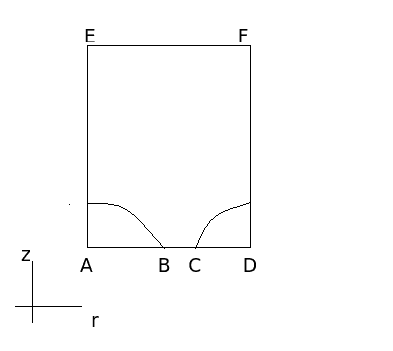
\includegraphics[scale=0.5]{figs/geometricbcs}
   \caption{Geometry}
\end{figure}
\begin{itemize}
\item $AB$ is the inlet
\item $BC$ is the thickness of the burner tube
\item $CD$ is the outside of the burner
\item $DE,EF$ is the domain of interest
\item $AE$ is the Axisymmetric line
\end{itemize}

\bigskip
\noindent The following assumption are made
\begin{itemize}
\item At the inlet, the incoming velcity has parabolic profile. i.e poissuelle flow. 
\item The surface chemistry at the wall of the burner is neglected. 
\item At the outside of the burner, the incoming air has couette flow profile. 
\item $DE,EF$ are the boundaries of the domain. No change occurs after this point. 
\end{itemize}
	
\noindent The boundary conditions are defined as follows 
\bigskip

\noindent At the inlet ($AB$)
\begin{itemize}
\item $u_r = 0$ and $u_z=5801.9 mm/s$
\item $C_i = 1$ 
\item $T = 300K$
\item $p=1 atmos$
\end{itemize}

\bigskip 
\noindent On $BC$
\begin{itemize}
\item $u_r = 0$ and $u_z=0 mm/s$
\item $\frac{\partial C_i}{\partial r} =0 $ and $\frac{\partial C_i}{\partial z} =0 $
\item $T = 300K$
\item $p=1 atmos$
\end{itemize}

\noindent On $CD$
\begin{itemize}
\item $u_r = 0$ and $u_z=5801.9 mm/s$
\item $ C_{O_2} =21 \% $
\item $T = 300K$
\item $p=1 atmos$
\end{itemize}

\noindent On $DF$ and $FE$
\begin{itemize}
\item $\frac{\partial u_r}{\partial r} =0 $ and $\frac{\partial u_z}{\partial z} =0 $
\item $\frac{\partial C_i}{\partial r} =0 $ and $\frac{\partial C_i}{\partial z} =0 $
\item $\frac{\partial T}{\partial r} =0 $ and $\frac{\partial T}{\partial z} =0 $
\item $\frac{\partial p}{\partial r} =0 $ and $\frac{\partial p}{\partial z} =0 $
\end{itemize}


\noindent On $AF$
\begin{itemize}
\item $\frac{\partial u_r}{\partial r} =0 $ 
\item $\frac{\partial C_i}{\partial r} =0 $ 
\item $\frac{\partial T}{\partial r} =0 $  
\item $\frac{\partial p}{\partial r} =0 $
\end{itemize}

\section{Transport Model}
\subsection{Viscocity}
\noindent We have used viscosity model as derived from kinetics theory under the ideal gas assumption
The kinetic theory uses the assumption of the ideal gas law.
 
$$pv = nRT$$ Where $p$ is the pressure, $v$ is the volume, $n$ is the number of moles of the gas, $R$ is the universal gas constant and $T$ is the temperature. The viscocity of the species is given by the following formula

$$\eta_s = \frac{5}{16}\sqrt{\frac{m_s k_B T}{\pi}}\frac{f_n}{{\sigma_s}^2   \Omega^{(2,2^*)}}$$

\noindent Where  $m$ the molecular mass of the species (kg), $\sigma$ is the Lennard-Jones potential diameter associated
to the species $(m)$, $k_B$ is the Boltzmann constant,$\Omega^{(2,2^*)}$ is the value of the dimensionless integrated integral from Monchick
and Mason (1961). With hard sphere approximation $f_n = 1$. We have three species in our system i.e $O$, $O_2$ and $O_3$. We have varied temperature from 300 K to 2700 K and plotted the viscocity V/s Temperature for all the three species. The $\sigma$ values and constants for dimensionless collision number are taken from NASA CAE transport file. 
\begin{figure}[H]
  \centering
  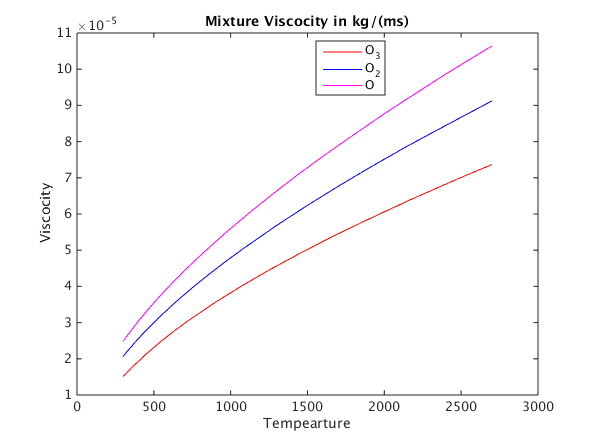
\includegraphics[scale=0.5]{figs/viscocity model.png}
   \caption{Viscocity}
\end{figure}

\subsection{Bimolecular Diffusion}
\noindent The molecular binary diffusion model is
computed from kinetics theory, assuming the ideal gas hypothesis. The molecular binary diffusion coefficient ($m^2 s^{-1}$ ) is given by:

$$D_{ij} = \frac{3}{16}\sqrt{\frac{2 k_B^3 T^3}{\pi m_{ij}}}\frac{f_n}{{ P \sigma_{ij}}^2   \Omega^{(1,1^*)}}$$

with  the reduced mass
\begin{equation}
m_{ij} = \left\{\begin{array}{l@{\qquad}l}
                \frac{m_i m_j}{m_i + m_j} &  i \neq j \\
                m_i                                  & i=j
                    \end{array}
              \right.
\end{equation}

$\sigma_{ij}$ is the Lennard-Jones collision diameter between species $i$ and $j$:
\begin{equation}
\sigma_{ij} = \frac{1}{2}\left(\sigma_i + \sigma_j\right) \xi^{-\frac{1}{6}}
\end{equation}

\noindent and $\Omega^{(1,1^*)}$ the integrated collision interval, fitted from the tables given in Monchick and Mason(1961). We have varied temperature from 300 K to 2700 K and plotted the Diffusion coefficient V/s Temperature for all the combination of three species. The $\sigma$ values and constants for dimensionless collision number are taken from NASA CAE transport file. 

\begin{figure}[H]

\subfloat[Diffusion coefficient for $O$ - $O$\label{subfig-1:dummy}]{%
     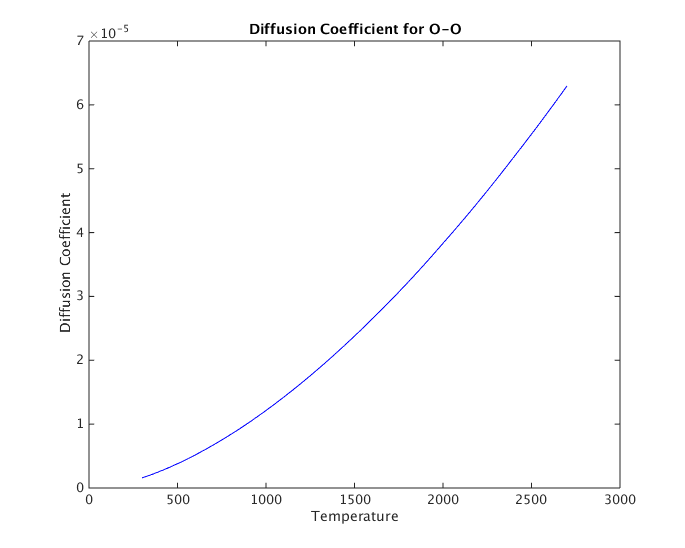
\includegraphics[scale=0.5]{figs/diffusionmodel00.png} 
    }
\subfloat[Diffusion coefficient for $O$ - $O_2$\label{subfig-1:dummy}]{%
     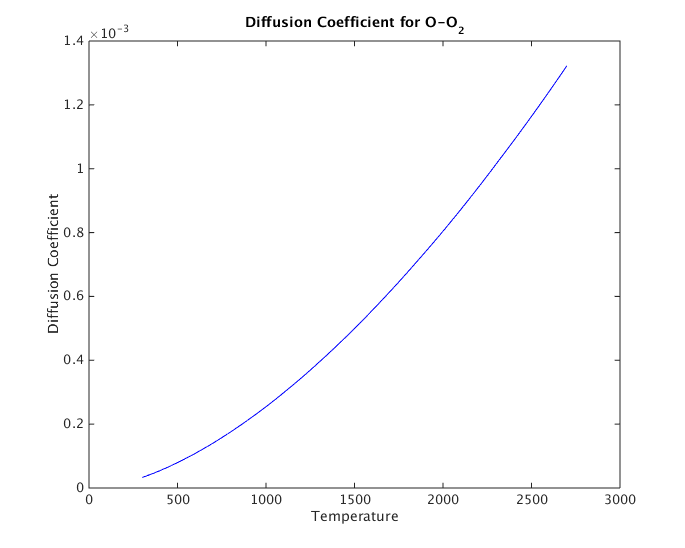
\includegraphics[scale=0.5]{figs/diffusionmodel002.png} 
    }
    \quad
   \subfloat[Diffusion coefficient for $O$ - $O_3$\label{subfig-1:dummy}]{%
        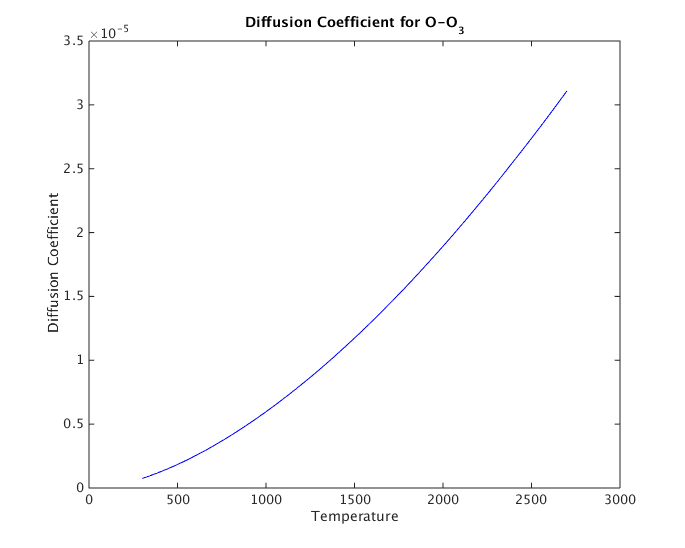
\includegraphics[scale=0.5]{figs/diffusionmodel003.png} 
       }
  \subfloat[Diffusion coefficient for $O_2$ - $O_2$\label{subfig-1:dummy}]{%
         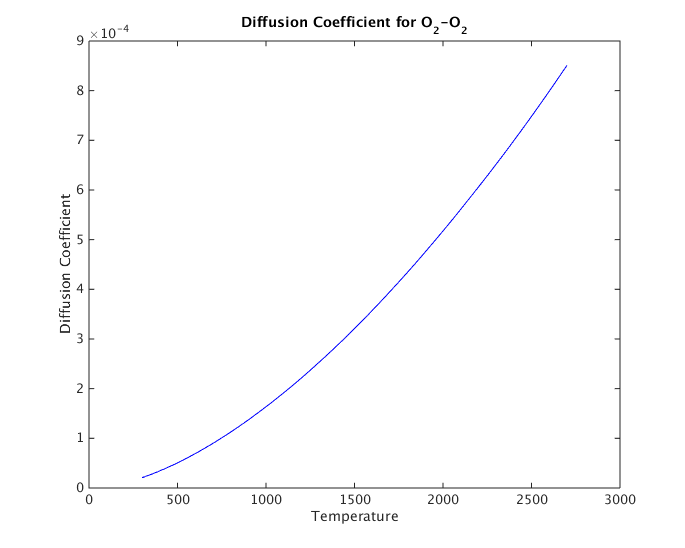
\includegraphics[scale=0.5]{figs/diffusionmodel0202.png} 
        }
        
        \quad
        \subfloat[Diffusion coefficient for $O_2$ - $O_3$\label{subfig-1:dummy}]{%
                 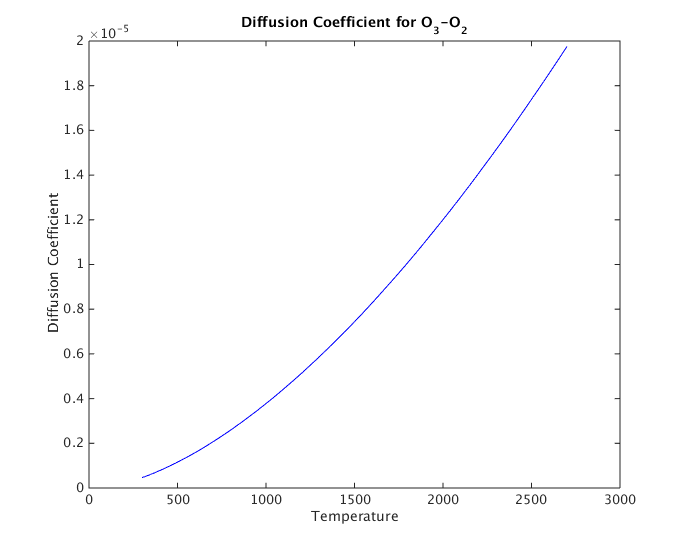
\includegraphics[scale=0.5]{figs/diffusionmodel0203.png} 
                }
         \subfloat[Diffusion coefficient for $O_3$ - $O_3$\label{subfig-1:dummy}]{%
            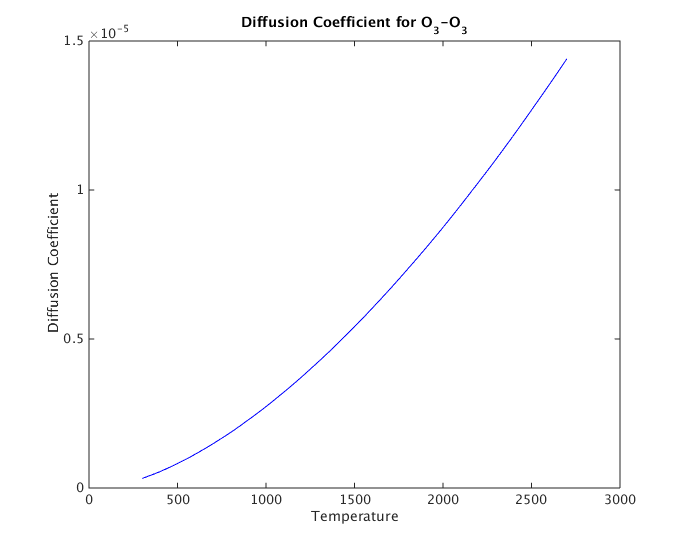
\includegraphics[scale=0.48]{figs/diffusionmodel0303.png} 
                                }
    \caption{Diffusion coefficient}
\end{figure}



\subsection{Species Thermal Conductivity}

The thermal conduction of a species $i$ is given by
\begin{eqnarray*}
\lambda_i &=& \lambda_i^{(\textnormal{rot})} + \lambda_i^{(\textnormal{trans})} + \lambda_i^{(\textnormal{vib})} \\
\lambda_i &=& \frac{\eta_i}{M_i} \left(
                        C_{v,i}^{(\textnormal{trans})} \lambda_i^{(\textnormal{trans})} + C_{v,i}^{(\textnormal{rot})} \lambda_i^{(\textnormal{rot})}+ C_{v,i}^{(\textnormal{vib})}  \lambda_i^{(\textnormal{vib})} 
                                          \right)
\end{eqnarray*}
with
%%
\begin{eqnarray*}
\lambda_{v,i}^{(\textnormal{vib})}   & =& \rho_i \frac{D_{i,i}}{\eta_i} \\
\lambda_{v,i}^{(\textnormal{rot})}   & =& \rho_i \frac{D_{i,i}}{\eta_i}\left(1 + \frac{2}{\pi}\frac{A}{B}\right) \\
\lambda_{v,i}^{(\textnormal{trans})}   & =&  \frac{5}{2} \left(1 - \frac{2}{\pi}\frac{C_{v,i}^{(\textnormal{rot})}}{C_{v,i}^{(\textnormal{trans})}}\frac{A}{B}\right)
\end{eqnarray*}
%
and
%
\begin{eqnarray*}
  A & = & \frac{5}{2} -  \rho_i \frac{D_{i,i}}{\eta_i}  \\
  B & = & Z_{rot} + \frac{2}{\pi} \left(\frac{5}{3}\frac{C_{v,i}^{(\textnormal{rot})}}{R} + \rho_i \frac{D_{i,i}}{\eta_i}\right)
\end{eqnarray*}
%
\noindent the rotational relaxation number is given by
\begin{equation}
Z_{rot,i}(T) = Z_{rot,i}(298)\frac{F(298)}{F(T)}
\label{thermal_cond:Zrot}
\end{equation}
\noindent with the function $F$ defined as
\begin{equation}
F(T) = 1 + \frac{\pi^{\frac{3}{2}}}{2}\sqrt{\left(\frac{\epsilon_i}{k_B T}\right)}
         + \left(\frac{\pi^2}{4} + 2\right)\left(\frac{\epsilon_i}{k_B T}\right)
         + \pi^{\frac{3}{2}}\left(\frac{\epsilon_i}{k_B T}\right)^{\frac{3}{2}}
\end{equation}

\noindent The specific heat are given by the thermodynamic module.  We have varied temperature from 300 K to 2700 K and plotted the thermal conductivity V/s Temperature for all the  three species. The $\sigma$ values and constants for dimensionless collision number are taken from NASA CAE transport file.

\begin{figure}[H]

\subfloat[Thermal Conductivity for $O$\label{subfig-1:dummy}]{%
     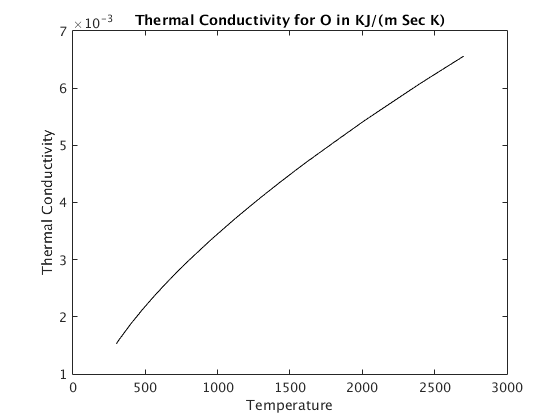
\includegraphics[scale=0.5]{figs/tcO.png} 
    }
\subfloat[Thermal Conductivity for $O_2$\label{subfig-1:dummy}]{%
     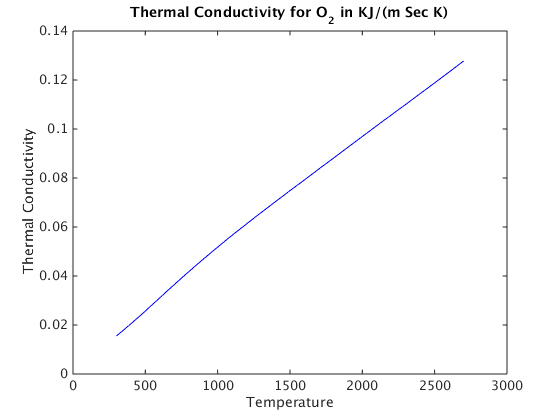
\includegraphics[scale=0.5]{figs/tcO2.png} 
    }
    \quad
   \subfloat[Thermal Conductivity for $O_3$\label{subfig-1:dummy}]{%
        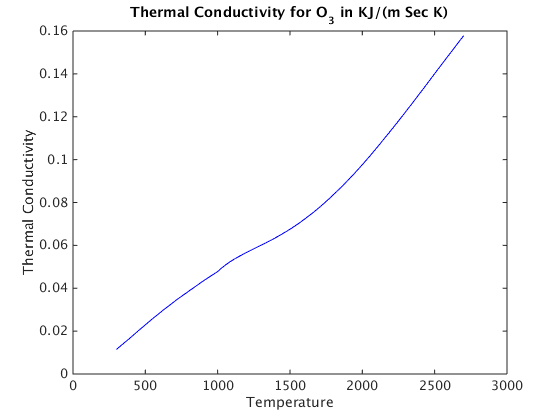
\includegraphics[scale=0.5]{figs/tcO3.png} 
       }
    \caption{Thermal Conductivity}
\end{figure}


\subsection{Mixture Model}
\noindent The Wilke formula for viscosity, independent of
the viscocity model, is
\begin{equation}
\eta_{\textnormal{mixture}} = \sum_{s=1}^{n} \frac {x_i \eta_i}{\sum_{j=1}^{n} x_j \Phi_{ij}}
\end{equation}
with
\begin{equation}
\Phi_{ij} = \frac{
                \left[
                     1 + \sqrt{\frac{\eta_i}{\eta_j}\sqrt{\frac{M_j}{M_i}}}
                \right]^2
                }{\sqrt{8\left(1 + \frac{M_i}{M_j}\right)}}
\end{equation}
\noindent  We have varied temperature from 300 K to 2700 K and plotted the mixture viscocity V/s Temperature for all the  three species. The $\sigma$ values and constants for dimensionless collision number are taken from NASA CAE transport file. We have considered three cases-  behind the flame where condentration of $O_3$,$O_2$ and $O$ are taken to be .53, .47 and 0 respectively. Second case of the inside of the flame where concentrations are 0.5, 0.4 and 0.1 respectively. The third case is of the behind the flame where ozone and oxygen radical are absent and there will be only $O_2$




\begin{figure}[H]

\subfloat[Mixture Viscocity behind the flame\label{subfig-1:dummy}]{%
     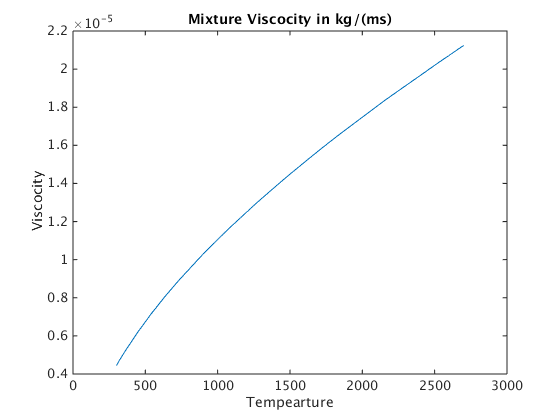
\includegraphics[scale=0.5]{figs/mixtureviscocty_behindflame.png} 
    }
\subfloat[Mixture Viscocity inside the flame\label{subfig-1:dummy}]{%
     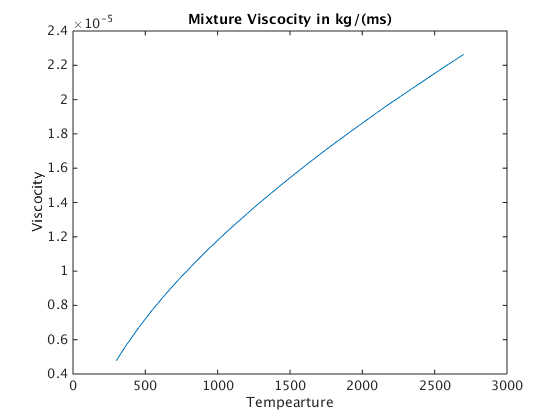
\includegraphics[scale=0.5]{figs/mixtureviscocty_insideflame.png} 
    }
    \quad
   \subfloat[Mixture Viscocity after the flame \label{subfig-1:dummy}]{%
        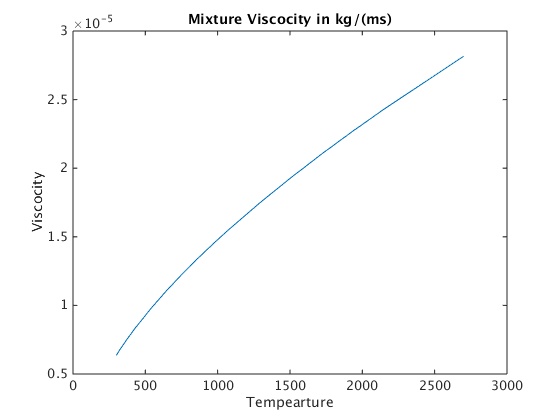
\includegraphics[scale=0.5]{figs/mixtureviscocty_afterflame.png} 
       }
    \caption{Mixture Viscocity}
\end{figure}


\noindent For the bimolecular diffusion model, we use:
\begin{equation}
D_i = \frac{1-y_i}{\sum_{j\ne i}^{n}\frac{x_i}{D_{ji}}}
         = \frac{\sum_{j\neq i}^{n} x_j M_j}{M_{\textnormal{mixture}} \sum_{j\ne i}^{n}\frac{x_j}{D_{ji}}}
\end{equation}

\begin{figure}[H]

\subfloat[Mixture Diffusion coefficient for $O_3$ behind the flame\label{subfig-1:dummy}]{%
     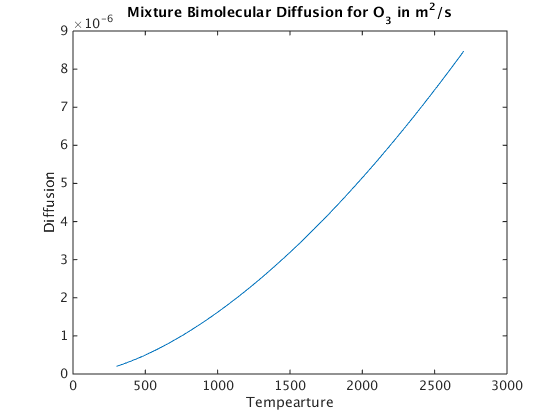
\includegraphics[scale=0.5]{figs/mixturediffusionO3_behindflame.png} 
    }
\subfloat[Mixture Diffusion coefficient for $O_2$ behind the flame\label{subfig-1:dummy}]{%
     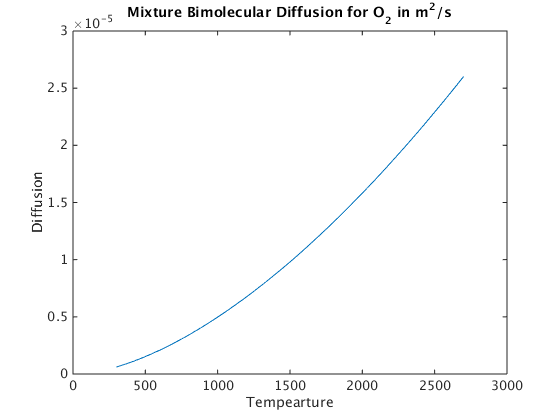
\includegraphics[scale=0.5]{figs/mixturediffusionO2_behindflame.png} 
    }
    \quad
   \subfloat[Mixture Diffusion coefficient for $O_3$ inside the flame\label{subfig-1:dummy}]{%
        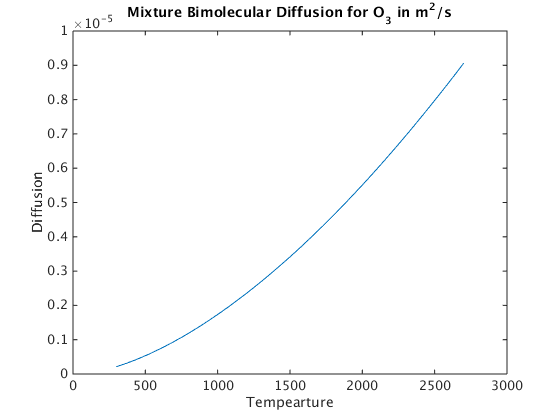
\includegraphics[scale=0.5]{figs/mixturediffusionO3_inflame.png} 
       }
  \subfloat[Mixture Diffusion coefficient for $O$ inside the flame\label{subfig-1:dummy}]{%
         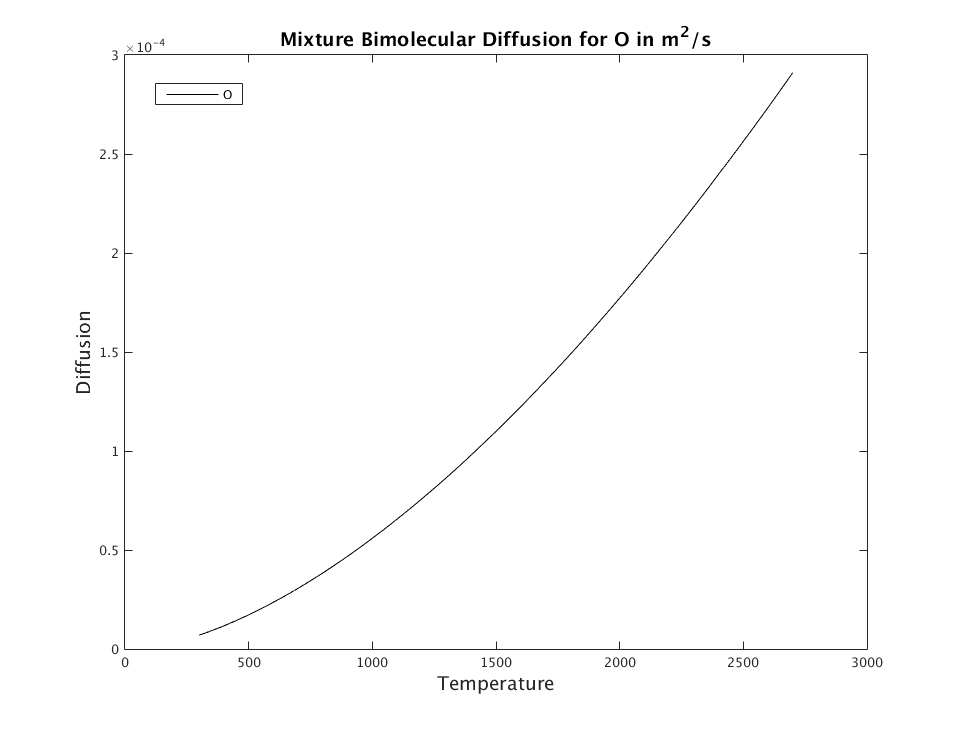
\includegraphics[scale=0.5]{figs/mixturediffusionO_inflame.png} 
        }
        
        \quad
        \subfloat[Mixture Diffusion coefficient for $O_2$ inside the flame - $O_3$\label{subfig-1:dummy}]{%
                 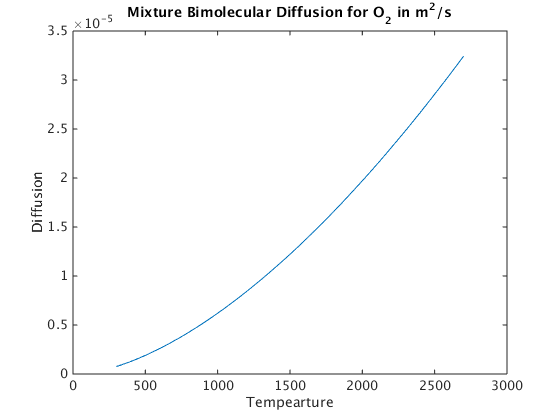
\includegraphics[scale=0.5]{figs/mixturediffusionO2_inflame.png} 
                }
         \subfloat[Mixture Diffusion coefficient for $O_2$ after the flame - $O_3$\label{subfig-1:dummy}]{%
            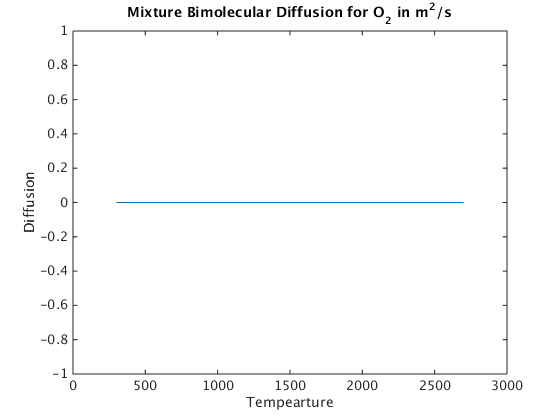
\includegraphics[scale=0.48]{figs/mixturediffusionO2_afterflame.png} 
                                }
    \caption{Mixture Diffusion coefficient}
\end{figure}


\noindent The thermal conductivity of the mixture is given by 
\begin{equation}
\lambda_{\textnormal{mixture}} = \sum_{s=1}^{n} \frac {x_i \lambda_i}{\sum_{j=1}^{n} x_j \Phi_{ij}}
\end{equation}
\noindent  We have varied temperature from 300 K to 2700 K and plotted the mixture thermal conductivity V/s Temperature for all the  three species. The $\sigma$ values and constants for dimensionless collision number are taken from NASA CAE transport file. We have considered three cases-  behind the flame where condentration of $O_3$,$O_2$ and $O$ are taken to be .53, .47 and 0 respectively. Second case of the inside of the flame where concentrations are 0.5, 0.4 and 0.1 respectively. The third case is of the behind the flame where ozone and oxygen radical are absent and there will be only $O_2$


\begin{figure}[H]

\subfloat[Mixture thermal conductivity behind the flame\label{subfig-1:dummy}]{%
     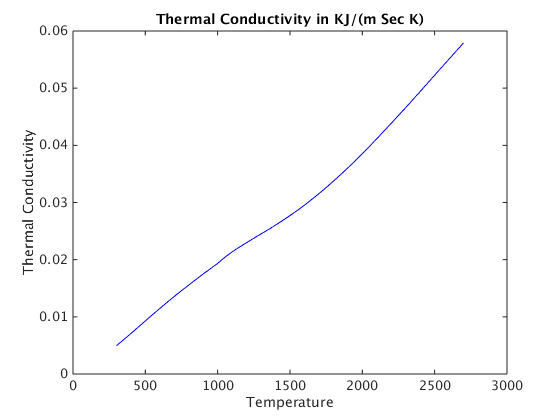
\includegraphics[scale=0.5]{figs/mixturethermal_behindflame.png} 
    }
\subfloat[Mixture thermal conductivity inside the flame\label{subfig-1:dummy}]{%
     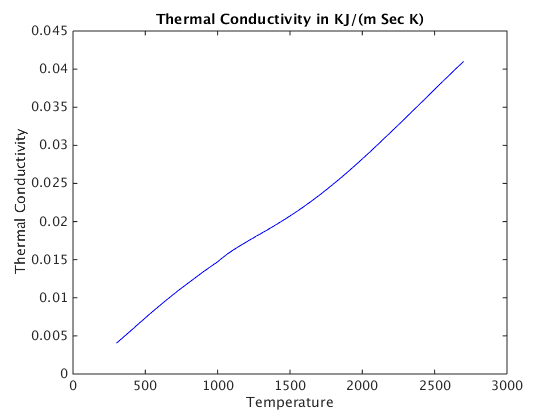
\includegraphics[scale=0.5]{figs/mixturethermal_insideflame.png} 
    }
    \quad
   \subfloat[Mixture thermal conductivity after the flame \label{subfig-1:dummy}]{%
        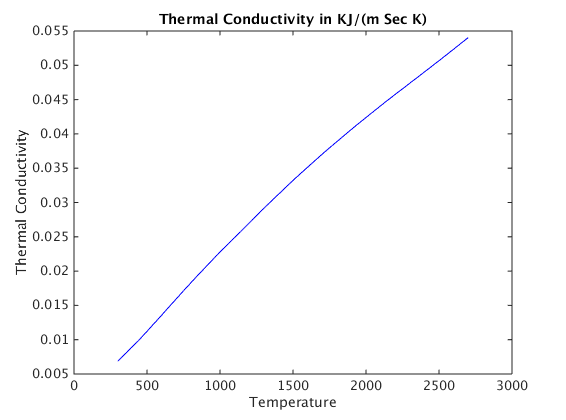
\includegraphics[scale=0.5]{figs/mixturethermal_afterflame.png} 
       }
    \caption{Mixture thermal conductivity}
\end{figure}
